\chapter{Difracción de Fraunhofer y filtrado espacial}\label{ch:b2:diffraction}

Mírese de reojo una farola por el hueco entre dos dedos y la farola se
estira en una banda de franjas; mírese una estrella por el mejor
telescopio y no se ve un punto, sino un pequeño disco rodeado de círculos
tenues. La luz que pasa por una abertura se abre --- cuanto más estrecha
la abertura, más se abre --- y ninguna lente puede concentrarla más de lo
que esa apertura permite. Esto es la \emph{\omterm{def:b2:diffraction:huygens}{difracción}}, la razón de que un
microscopio no pueda ver un virus, de que el poder resolvente de un
telescopio crezca con su diámetro y de que un haz láser no pueda seguir
paralelo. Este capítulo calcula el patrón de \omterm{def:b2:diffraction:huygens}{difracción} de una abertura en
el campo lejano, el límite que impone a todo instrumento óptico, cómo se
combina con las interferencias y la idea --- la de Abbe --- que convierte
el plano focal de una lente en un lugar donde puede filtrarse una imagen.

\section{El principio de Huygens--Fresnel y el régimen de Fraunhofer}

\begin{definition}[Principio de Huygens--Fresnel]\label{def:b2:diffraction:huygens}
\index{principio de Huygens--Fresnel}\index{difracción}\index{difracción de Fraunhofer}
Todo punto de un \omterm{def:b2:scalar-light-model:path}{frente de onda} (o de una abertura iluminada por una onda) actúa como
fuente secundaria que emite una ondícula esférica, en fase con la onda
allí; la onda de más allá es la suma coherente de las ondículas. Para una
abertura $\Sigma$ iluminada por una onda plana de amplitud $a$, la amplitud
que llega a un punto lejano vale $\underline s(M) = K\iint_\Sigma\eu^{-\iu\varphi(P, M)}\dd S$, con
$\varphi(P, M)$ la fase del camino del punto $P$ de la abertura hasta $M$
($K$ una constante). La difracción de \emph{Fraunhofer} (de campo lejano) es el caso
en que $M$ está en el infinito --- o en el plano focal de una lente --- de modo que
los rayos que van de todos los puntos de la abertura hacia $M$ son paralelos, en
la dirección $\vect u$, y
\[
\varphi(P, M) = \varphi_0 - \frac{2\pi}\lambda\,\vect{OP}\cdot\vect u , \qquad
\underline s(\vect u) \propto \iint_\Sigma\eu^{\iu(2\pi/\lambda)\vect{OP}\cdot\vect u}\dd S .
\]
El patrón se observa en el infinito, o en el foco $F'$ de una lente,
donde la dirección $\vect u$ de ángulos pequeños $(\alpha, \beta)$ corresponde al
punto $(f\alpha, f\beta)$.
\end{definition}
\admitted

\begin{remark}[¿Cuándo está bastante lejos?]\label{rem:b2:diffraction:fresnelnumber}
\index{número de Fresnel}
Para una abertura de tamaño $D$ vista a la distancia $L$ sin lente, los
rayos son bastante paralelos cuando el término cuadrático de
\cref{exo:b2:scalar-light-model:12} es despreciable, $D^2/L \ll \lambda$ ---
el \emph{\omterm{rem:b2:diffraction:fresnelnumber}{número de Fresnel}} $D^2/\lambda L \ll 1$. Una rendija de \qty{0.1}{mm} a
\qty{500}{nm} exige $L \gg \qty{2}{cm}$; una abertura de \qty{1}{cm}, $L \gg \qty{200}{m}$ ---
de ahí la lente, que trae el infinito a su plano focal. Más cerca
(\omterm{def:b2:diffraction:huygens}{difracción} de Fresnel) los patrones son más complejos; la sombra de un
borde recto, por ejemplo, tiene franjas por su lado iluminado.
\end{remark}

\section{La rendija única y la abertura circular}

\begin{proposition}[Difracción por una rendija]\label{prop:b2:diffraction:slit}
\index{difracción por una rendija}\index{función sinc}
Una rendija de anchura $b$ (alargada según $y$) iluminada con incidencia normal envía en
la dirección $\theta$ (en el plano perpendicular a la rendija) la
intensidad
\[
I(\theta) = I_0\,\operatorname{sinc}^2\Bigl(\frac{\pi b\sin\theta}\lambda\Bigr) , \qquad \operatorname{sinc}x = \frac{\sin x}x :
\]
un máximo central brillante de semianchura angular $\lambda/b$ (primeros ceros en
$\sin\theta = \pm\lambda/b$), que contiene el $90\%$ de la luz, y \omterm{thm:b2:gratings:nwaves}{máximos secundarios}
en torno a $\sin\theta = \pm1.43\lambda/b$, $\pm2.46\lambda/b$, \dots, de intensidades
relativas $4.7\%$, $1.6\%$, \dots --- cuanto más estrecha la rendija, más ancho
el patrón. En el plano focal de una lente de distancia focal $f$ el
máximo central mide $2\lambda f/b$ de ancho.
\end{proposition}

\begin{proof}
$\underline s(\theta) \propto \int_{-b/2}^{b/2}\eu^{\iu kx\sin\theta}\dd x = b\,\operatorname{sinc}(kb\sin\theta/2)$
con $k = 2\pi/\lambda$; elévese al cuadrado. Hay ceros donde $b\sin\theta = m\lambda$, $m \ne 0$: las
ondículas de las dos mitades de la rendija se cancelan entonces dos a dos.
\end{proof}

\begin{omfigure}
\begin{tikzpicture}[font=\small, x=1cm, y=1cm, >=Stealth]
  \begin{scope}
    \draw[thick] (0,-2) -- (0,-0.5) (0,0.5) -- (0,2);
    \draw[<->] (-0.35,-0.5) -- (-0.35,0.5) node[midway, left, font=\footnotesize] {$b$};
    \foreach \y in {-1.6,-0.9,-0.2,0.5,1.2} \draw[omDef, ->] (-2.2,\y) -- (-0.1,\y);
    \foreach \y in {-0.4,-0.2,0,0.2,0.4} \draw[omThm, thick, ->] (0.1,\y) -- (2.4,{\y+1.0});
    \draw[dashed] (0.1,0) -- (2.6,0); \draw (1.4,0) arc[start angle=0, end angle=23.5, radius=1.4]; \node[font=\footnotesize] at (1.7,0.28) {$\theta$};
    \node[font=\footnotesize] at (1.2,-1.6) {$b\sin\theta = \lambda$: primer cero};
  \end{scope}
  \begin{scope}[xshift=8.6cm]
    \begin{axis}[omaxis, axis x line=bottom, axis y line=left, width=6.4cm, height=4.4cm, at={(0,-2.0cm)},
        xlabel={$b\sin\theta/\lambda$}, ylabel={$I/I_0$}, xmin=-3.2, xmax=3.2, ymin=0, ymax=1.1, xtick={-3,-2,-1,0,1,2,3}, ytick={0.5,1}, samples=400,
        xlabel style={at={(axis description cs:0.5,-0.14)}, anchor=north},
        ylabel style={at={(axis description cs:-0.1,0.5)}, rotate=90, anchor=south}]
      \addplot[omDef, thick, domain=-3.2:3.2] {(sin(deg(pi*x))/(pi*x+1e-9))^2};
    \end{axis}
  \end{scope}
\end{tikzpicture}

{\small A la izquierda, las ondículas de toda la rendija, sumadas en la dirección
$\theta$. A la derecha, el patrón de Fraunhofer de la rendija, $\operatorname{sinc}^2$: un
lóbulo central el doble de ancho que los demás y mucho más brillante.}
\end{omfigure}

\begin{proposition}[Abertura circular; el disco de Airy]\label{prop:b2:diffraction:airy}
\index{disco de Airy}\index{criterio de Rayleigh (resolución)}\index{poder resolvente (instrumento)}
Una abertura circular de diámetro $D$ da un disco central brillante, el
\emph{\omterm{prop:b2:diffraction:airy}{disco de Airy}}, rodeado de anillos tenues; el primer anillo oscuro está en
\[
\sin\theta = 1.22\,\frac\lambda D ,
\]
y el disco contiene el $84\%$ de la luz. Todo instrumento con una
pupila de entrada de diámetro $D$ --- ojo, cámara, telescopio, objetivo de
microscopio --- convierte una fuente puntual en un \omterm{prop:b2:diffraction:airy}{disco de Airy} de ese radio
angular; dos puntos quedan \emph{resueltos} (criterio de Rayleigh) si su
separación angular supera $1.22\lambda/D$: el poder resolvente del
instrumento.
\end{proposition}
\admitted

\begin{example}[Ojo, telescopio, microscopio]\label{ex:b2:diffraction:instruments}
El ojo ($D = \qty{3}{mm}$, $\lambda = \qty{550}{nm}$): $1.22\lambda/D = \qty{2.2e-4}{rad}$, unos
\qty{45}{''} --- un detalle de \qty{1}{mm} a \qty{4}{m}, que es en efecto más o menos la
agudeza de un buen ojo: la evolución ajustó las células de la retina al
límite de \omterm{def:b2:diffraction:huygens}{difracción}. Un telescopio de \qty{2.4}{m}: \qty{0.06}{''}, mil veces
mejor, si la atmósfera lo permite (no lo permite desde el suelo:
\qty{1}{''} de ``seeing'', de donde los telescopios espaciales y la óptica adaptativa). Una
antena de radio de \qty{100}{m} a $\lambda = \qty{21}{cm}$: \qty{9}{'}, peor que el ojo;
los interferómetros entre continentes recuperan la resolución. Un
objetivo de microscopio de ángulo de abertura $\alpha$ resuelve $0.61\lambda/n\sin\alpha$
--- unos \qty{0.2}{\micro m} en el visible, sea cual sea el aumento: el
límite que llevó la microscopía a los electrones y a los rayos X.
\end{example}

\begin{omfigure}
\begin{tikzpicture}[font=\small, x=1cm, y=1cm]
  \begin{scope}
    \foreach \r/\g in {1.5/85, 1.25/70, 1.0/50, 0.8/25, 0.6/5, 0.45/40, 0.3/70, 0.15/95} {
      \fill[black!\g] (0,0) circle (\r);
    }
    \node[font=\footnotesize] at (0,-1.9) {patrón de Airy de una estrella};
  \end{scope}
  \begin{scope}[xshift=4.2cm]
    \foreach \r/\g in {0.8/25, 0.6/5, 0.45/40, 0.3/70, 0.15/95} {
      \fill[black!\g] (-0.45,0) circle (\r);
    }
    \foreach \r/\g in {0.8/25, 0.6/5, 0.45/40, 0.3/70, 0.15/95} {
      \fill[black!\g, opacity=0.6] (0.45,0) circle (\r);
    }
    \node[font=\footnotesize] at (0,-1.9) {dos estrellas en el límite de Rayleigh};
  \end{scope}
  \begin{scope}[xshift=9.6cm]
    \begin{axis}[omaxis, axis x line=bottom, axis y line=left, width=5.4cm, height=4.0cm, at={(0,-1.8cm)},
        xlabel={$\theta D/\lambda$}, ylabel={$I$}, xmin=-2.5, xmax=3.5, ymin=0, ymax=1.5, xtick={-1.22,0,1.22,2.44}, xticklabels={$-1.22$,$0$,$1.22$,$2.44$}, ytick=\empty, samples=300,
        xlabel style={at={(axis description cs:0.5,-0.14)}, anchor=north},
        ylabel style={at={(axis description cs:-0.06,0.5)}, rotate=90, anchor=south}]
      \addplot[omDef, thick, domain=-2.5:3.5] {(sin(deg(pi*x/1.22))/(pi*x/1.22+1e-9))^2};
      \addplot[omThm, thick, domain=-2.5:3.5] {(sin(deg(pi*(x-1.22)/1.22))/(pi*(x-1.22)/1.22+1e-9))^2};
    \end{axis}
  \end{scope}
\end{tikzpicture}

{\small A la izquierda y en el centro: el \omterm{prop:b2:diffraction:airy}{disco de Airy} de una fuente puntual y dos
fuentes en el límite de Rayleigh --- el centro de una sobre el primer anillo
oscuro de la otra. A la derecha, sus perfiles (esbozados con formas
$\operatorname{sinc}^2$), separados $1.22\lambda/D$.}
\end{omfigure}

\section{Difracción e interferencias juntas}

\begin{proposition}[Rendijas de Young de anchura finita; la envolvente de la red]\label{prop:b2:diffraction:combined}
\index{envolvente (difracción)}\index{órdenes ausentes}
Dos rendijas de anchura $b$ cuyos centros distan $a$ dan
\[
I(\theta) = 4I_0\,\operatorname{sinc}^2\Bigl(\frac{\pi b\sin\theta}\lambda\Bigr)\cos^2\Bigl(\frac{\pi a\sin\theta}\lambda\Bigr) :
\]
las franjas de Young (separadas $\lambda/a$ en $\sin\theta$) bajo la envolvente de una
sola rendija (de anchura $2\lambda/b$); $a/b$ franjas llenan el lóbulo central, y las
franjas en $a\sin\theta = p\lambda$ que caen sobre un cero de la envolvente
($b\sin\theta = m\lambda$) están \emph{ausentes}. Una red de $N$ rendijas de anchura
$b$ tiene igualmente sus \omterm{thm:b2:gratings:nwaves}{máximos principales} modulados por la misma envolvente ---
que el blaze de \cref{ch:b2:gratings} inclina hacia el orden que se usa.
\end{proposition}

\begin{proof}
La integral de abertura se separa en una suma sobre las dos rendijas de la misma
integral desplazada en $\pm a/2$: $\underline s \propto b\,\operatorname{sinc}(\pi b\sin\theta/\lambda)
\times2\cos(\pi a\sin\theta/\lambda)$. Para $N$ rendijas, el segundo factor es la
suma de $N$ ondas.
\end{proof}

\begin{omfigure}
\begin{tikzpicture}
\begin{axis}[omaxis, axis x line=bottom, axis y line=left, width=13.6cm, height=4.6cm,
    xlabel={$a\sin\theta/\lambda$}, ylabel={$I/4I_0$}, xmin=-9, xmax=9, ymin=0, ymax=1.1, xtick={-8,-4,0,4,8}, ytick={0.5,1}, samples=1200,
    xlabel style={at={(axis description cs:0.5,-0.12)}, anchor=north},
    ylabel style={at={(axis description cs:-0.04,0.5)}, rotate=90, anchor=south}]
  \addplot[omDef, thick, domain=-9:9] {(sin(deg(pi*x/4))/(pi*x/4+1e-9))^2*cos(deg(pi*x))^2};
  \addplot[omThm, thick, dashed, domain=-9:9] {(sin(deg(pi*x/4))/(pi*x/4+1e-9))^2};
\end{axis}
\end{tikzpicture}

{\small Dos rendijas con $a = 4b$: franjas de Young bajo la envolvente de una
sola rendija (discontinua); las franjas de cuarto orden caen sobre los ceros de la
envolvente y faltan.}
\end{omfigure}

\section{El plano de Fourier y el filtrado espacial}

\begin{proposition}[La lente como analizador de Fourier]\label{prop:b2:diffraction:fourier}
\index{plano de Fourier}\index{frecuencia espacial}\index{filtrado espacial}\index{teoría de Abbe}
Una transparencia de transmitancia $t(x, y)$ en el plano focal objeto de una
lente, iluminada por una onda plana, produce en el plano focal imagen la
amplitud
\[
\underline s(X, Y) \propto \iint t(x, y)\,\eu^{-\iu2\pi(xX + yY)/\lambda f}\dd x\,\dd y
\]
--- su transformada de Fourier bidimensional, y cada punto $(X, Y)$ del
\emph{\omterm{prop:b2:diffraction:fourier}{plano de Fourier}} recoge la luz difractada en los ángulos
$(X/f, Y/f)$, es decir, las \emph{\omterm{prop:b2:diffraction:fourier}{frecuencias espaciales}} $(X/\lambda f, Y/\lambda f)$ del
objeto: los detalles finos (frecuencias altas) lejos del eje y los gruesos
cerca de él. Una segunda lente rehace la imagen a partir de ese plano; todo lo
que allí se bloquee o se altere queda filtrado de la imagen
(\emph{\omterm{prop:b2:diffraction:fourier}{filtrado espacial}}, \omterm{prop:b2:diffraction:fourier}{teoría de Abbe} del microscopio): un agujerito
en el eje conserva solo las frecuencias bajas (suavizado, ``limpieza'' de un
haz láser); un tope en el eje elimina el fondo uniforme y
conserva los bordes (campo oscuro, estrioscopia); una \omterm{prop:b2:plane-waves-polarization:plates}{lámina de cuarto de onda} en el
eje convierte los objetos de fase, invisibles de otro modo, en contraste de intensidad
(contraste de fase, Zernike).
\end{proposition}

\begin{proof}[Justificación]
En la integral de Fraunhofer, $\vect{OP}\cdot\vect u = x\alpha + y\beta$ con la
dirección llevada a $(X, Y) = (f\alpha, f\beta)$; la transmitancia pondera
cada fuente secundaria. (La propia transformada de Fourier se estudia en el
volumen de matemáticas del tercer año; aquí es solo el nombre de esta integral.)
Para un objeto periódico de periodo $d$ la transformada es el conjunto de los órdenes
de una red en $X = p\lambda f/d$: la imagen solo puede mostrar el periodo si al menos
los órdenes $\pm1$ pasan por la lente --- la condición de Abbe, que es
de nuevo el límite de resolución del microscopio.
\end{proof}

\begin{omfigure}
\begin{tikzpicture}[font=\small, x=1cm, y=1cm, >=Stealth]
  \draw[omDef, thick, ->] (-5.6,0.8) -- (-4.6,0.8); \draw[omDef, thick, ->] (-5.6,0) -- (-4.6,0); \draw[omDef, thick, ->] (-5.6,-0.8) -- (-4.6,-0.8);
  \draw[thick, fill=omExo!20] (-4.4,-1.4) rectangle (-4.3,1.4); \node[font=\footnotesize] at (-4.35,-1.75) {objeto $t(x, y)$};
  \draw[thick, fill=omExo!20] (-2.4,0) ellipse (0.2 and 1.5); \node[font=\footnotesize] at (-2.4,-1.85) {$L_1$};
  \draw[thick] (0,-1.4) -- (0,1.4); \fill[omThm] (0,0) circle (2pt); \fill[omThm] (0,0.7) circle (1.5pt); \fill[omThm] (0,-0.7) circle (1.5pt);
  \node[font=\footnotesize] at (0,-1.75) {plano de Fourier};
  \draw[thick, fill=omExo!20] (2.4,0) ellipse (0.2 and 1.5); \node[font=\footnotesize] at (2.4,-1.85) {$L_2$};
  \draw[thick, fill=omExo!20] (4.3,-1.4) rectangle (4.4,1.4); \node[font=\footnotesize] at (4.35,-1.75) {imagen};
  \draw[omThm] (-4.35,0.6) -- (-2.4,1.0) -- (0,0.7) -- (2.4,0.4) -- (4.35,-0.6);
  \draw[omThm] (-4.35,-0.6) -- (-2.4,-1.0) -- (0,-0.7) -- (2.4,-0.4) -- (4.35,0.6);
  \draw[omProp] (-4.35,0.6) -- (-2.4,0.6) -- (0,0) -- (2.4,-0.6) -- (4.35,-0.6);
  \draw[omProp] (-4.35,-0.6) -- (-2.4,-0.6) -- (0,0) -- (2.4,0.6) -- (4.35,0.6);
  \draw[<->] (-4.35,1.7) -- (-2.4,1.7) node[midway, above, font=\footnotesize] {$f$}; \draw[<->] (-2.4,1.7) -- (0,1.7) node[midway, above, font=\footnotesize] {$f$};
  \node[omThm, font=\footnotesize, anchor=west] at (0.15,0.95) {órdenes de un objeto periódico};
\end{tikzpicture}

{\small El montaje $4f$: la primera lente forma la transformada de
Fourier del objeto en su plano focal (un objeto periódico da allí
órdenes discretos) y la segunda rehace la imagen; una máscara en el
\omterm{prop:b2:diffraction:fourier}{plano de Fourier} filtra la imagen.}
\end{omfigure}

\begin{example}[Limpiar un haz, ver lo invisible]\label{ex:b2:diffraction:filtering}
Un haz láser lleva polvo y ondulaciones: enfóquese por un agujerito de
unos pocos micrómetros --- el tamaño del \omterm{prop:b2:diffraction:airy}{disco de Airy} central del haz
gaussiano limpio --- y todo lo demás, que queda fuera, se bloquea;
el haz recolimado es liso: un \emph{filtro espacial}. Una célula viva
es transparente; solo cambia la fase de la luz. Bloquear la mancha
axial hace brillar sus bordes sobre negro; la lámina de Zernike
retrasa un cuarto de onda la luz no difractada para que interfiera
con la difractada en intensidad: aparece el interior de la célula
y la biología consiguió su microscopio (premio Nobel de 1953).
\end{example}

\begin{method}[Estimaciones de difracción]\label{met:b2:diffraction:method}
(1) Apertura angular $\sim\lambda/b$ para una abertura de tamaño $b$ ($1.22\lambda/D$ para
un círculo); el tamaño del patrón a la distancia $L$ o con distancia focal $f$ vale
$\lambda L/b$, $\lambda f/b$. (2) Compruébese la condición de Fraunhofer $b^2/\lambda L \ll 1$ o
úsese una lente. (3) Combínense: envolvente de \omterm{def:b2:diffraction:huygens}{difracción} $\times$ franjas de
interferencia. (4) Resolución: dos puntos exigen $\Delta\theta > 1.22\lambda/D$; un objeto
periódico exige que sus primeros órdenes entren en la pupila. (5) La imagen del
\omterm{prop:b2:diffraction:fourier}{plano de Fourier}: qué bloquear para eliminar qué detalle.
\end{method}

\section{Ejercicios}

\begin{exercise}[$\star$]\label{exo:b2:diffraction:1}
Una rendija de \qty{0.10}{mm} iluminada por un láser de He--Ne (\qty{633}{nm}); pantalla a
\qty{2.0}{m}. Anchura del máximo central; posición de los dos primeros
\omterm{thm:b2:gratings:nwaves}{máximos secundarios}; \omterm{rem:b2:diffraction:fresnelnumber}{número de Fresnel} --- ¿está la pantalla bastante lejos? La misma
rendija con una lente de $f = \qty{50}{cm}$.
\end{exercise}

\begin{exercise}[$\star$]\label{exo:b2:diffraction:2}
Poder resolvente (Rayleigh) de: el ojo (\qty{3}{mm}, \qty{550}{nm}); un
telescopio de aficionado de \qty{10}{cm}; el espejo de \qty{2.4}{m} del Hubble; una antena
de radio de \qty{64}{m} a \qty{6}{cm}; un objetivo de cámara de \qty{50}{mm} a $f/8$ (pupila de \qty{6}{mm}):
tamaño del \omterm{prop:b2:diffraction:airy}{disco de Airy} en el sensor, comparado con un píxel de \qty{4}{\micro m}.
\end{exercise}

\begin{exercise}[$\star$]\label{exo:b2:diffraction:3}
Dos rendijas de anchura $b = \qty{0.05}{mm}$, con los centros separados $a = \qty{0.25}{mm}$, $\lambda =
\qty{500}{nm}$, lente $f = \qty{1}{m}$: separación de las franjas; anchura de la envolvente
central; número de franjas dentro; ¿qué órdenes faltan?
\end{exercise}

\begin{exercise}[$\star$]\label{exo:b2:diffraction:4}
Un haz láser de \qty{2}{mm} de diámetro a \qty{633}{nm} se propaga hasta la Luna
(\qty{3.8e8}{m}): ángulo de \omterm{def:b2:diffraction:huygens}{difracción} $\sim1.22\lambda/D$, diámetro de la mancha;
con un telescopio de \qty{3.5}{m} como emisor; ¿por qué son tan débiles los retornos de la
telemetría lunar (el retrorreflector, de \qty{1}{m}, devuelve la luz con su propia
\omterm{def:b2:diffraction:huygens}{difracción})?
\end{exercise}

\begin{exercise}[$\star\star$]\label{exo:b2:diffraction:5}
\emph{La rendija en detalle.} (a) Realícese la integral de Fraunhofer para
la rendija y obténgase $\operatorname{sinc}^2$. (b) Muéstrese que los \omterm{thm:b2:gratings:nwaves}{máximos secundarios}
están en $\tan x = x$ ($x = \pi b\sin\theta/\lambda$), el primero cerca de $x = 1.43\pi$, y
calcúlese su intensidad relativa. (c) Fracción de la energía en el
lóbulo central (admítanse $\int_{-\pi}^\pi\operatorname{sinc}^2 = 0.903\pi$ y
$\int_{-\infty}^\infty\operatorname{sinc}^2 = \pi$). (d) La rendija se ilumina con incidencia
$\theta_0$: muéstrese que el patrón es el mismo, centrado en la dirección $\theta_0$.
\end{exercise}

\begin{exercise}[$\star\star$]\label{exo:b2:diffraction:6}
\emph{Microscopio.} Un objetivo de \omterm{prop:b2:guided-waves:fibre}{apertura numérica} $n\sin\alpha = 1.4$
(inmersión en aceite) a \qty{500}{nm}: menor distancia resuelta $0.61\lambda/n\sin
\alpha$; con luz azul (\qty{400}{nm}); en el ultravioleta (\qty{250}{nm}); ¿por qué
no ayuda un ocular de $1000\times$ (el propio límite del ojo a \qty{25}{cm} es
\qty{0.1}{mm})? ¿Qué cambian los microscopios electrónicos ($\lambda = \qty{4}{pm}$ a
\qty{100}{keV})?
\end{exercise}

\begin{exercise}[$\star\star$]\label{exo:b2:diffraction:7}
\emph{Rectangular y circular.} (a) Una abertura rectangular $b \times h$:
muéstrese que el patrón vale $\operatorname{sinc}^2(\pi b\sin\theta_x/\lambda)\operatorname{sinc}^2(\pi h
\sin\theta_y/\lambda)$: una cruz, más ancha según el lado más estrecho. (b) Un cuadrado de
\qty{0.2}{mm} con $f = \qty{1}{m}$: tamaño del cuadrado central. (c) Para un
círculo de la misma anchura el primer cero está en $1.22\lambda/D$ en vez de $\lambda/b$:
¿por qué más lejos (piénsese en la luz concentrada cerca del centro de un
disco)? (d) El espejo secundario de un telescopio va sujeto por cuatro brazos: ¿qué
añaden a la imagen de una estrella brillante?
\end{exercise}

\begin{exercise}[$\star\star$]\label{exo:b2:diffraction:8}
\emph{Abbe.} Se observa una red de periodo $d = \qty{2}{\micro m}$ con un
objetivo de microscopio de ángulo de abertura $\alpha$ en aire, $\lambda = \qty{550}{nm}$.
(a) Ángulos de sus órdenes $\pm1$ y $\pm2$. (b) $\sin\alpha$ mínimo para que la imagen
muestre el periodo (deben entrar los órdenes $\pm1$). (c) Con $\sin\alpha = 0.4$: ¿qué
muestra la imagen; es una red fiel? (d) La iluminación oblicua deja pasar
el orden cero y \emph{un} primer orden:
$\sin\alpha$ mínimo entonces, y la ganancia.
\end{exercise}

\begin{exercise}[$\star\star$]\label{exo:b2:diffraction:9}
\emph{Filtro espacial.} Un haz láser de \qty{2}{mm} ($\lambda = \qty{633}{nm}$) se
enfoca con una lente de $f = \qty{20}{mm}$ a través de un agujerito. (a) Diámetro del
\omterm{prop:b2:diffraction:airy}{disco de Airy} central en el foco; diámetro del agujerito para dejarlo pasar
(tómese $1.5\times$). (b) Una mota de polvo de \qty{50}{\micro m} en el haz
difracta la luz ¿con qué ángulo, y dónde cae esa luz en el
plano focal: por el agujerito o no? (c) Potencia perdida si el haz
es gaussiano y el agujerito deja pasar el $99\%$; ¿por qué es liso el haz
que emerge? (d) ¿Por qué debe centrarse el agujerito con precisión de unos pocos
micrómetros?
\end{exercise}

\begin{exercise}[$\star\star\star$]\label{exo:b2:diffraction:10}
\emph{Babinet.} Dos pantallas complementarias (una rendija y una banda
opaca de la misma anchura) se iluminan con una onda plana. (a) Muéstrese que, fuera
de la dirección del haz incidente, sus patrones de Fraunhofer
son idénticos (la suma de las dos amplitudes es la de la
onda sin obstáculo, nula fuera del eje). (b) El patrón de un cabello de
\qty{80}{\micro m} de diámetro a \qty{2}{m} con un láser: separación de las franjas y
diámetro del cabello a partir de ella --- una medida estándar. (c) ¿Qué se ve
sobre el eje mismo? (d) ¿Por qué producen las gotitas de una nube fina una
corona de anillos coloreados en torno a la Luna, y qué da el radio de los
anillos?
\end{exercise}

\begin{exercise}[$\star\star\star$]\label{exo:b2:diffraction:11}
\emph{Campo oscuro y contraste de fase.} Un objeto transparente tiene
$t(x) = \eu^{\iu\varphi(x)} \approx 1 + \iu\varphi(x)$ con $|\varphi| \ll 1$. (a) Intensidad de
su imagen ordinaria: muéstrese que es uniforme a primer orden --- invisible. (b)
En el \omterm{prop:b2:diffraction:fourier}{plano de Fourier} el ``1'' es la mancha axial y $\iu\varphi$ la
luz difractada a su alrededor: si un tope bloquea la mancha axial, la intensidad de la
imagen vale $\propto\varphi^2$ --- campo oscuro; su debilidad. (c) Si en cambio la
mancha axial se retrasa $\pi/2$ (multiplicada por $\iu$): imagen $\propto|1 +
\varphi|^2 \approx 1 + 2\varphi$ --- contraste de fase, lineal en $\varphi$. (d) ¿Por qué la
lámina de Zernike suele además absorber (atenúa la mancha axial)?
\end{exercise}

\begin{exercise}[$\star\star\star$]\label{exo:b2:diffraction:12}
\emph{Resolución de la imagen de la rendija de un espectrógrafo y la red.} Una
red de anchura $W$ es la abertura del espectrógrafo: muéstrese que el
patrón de \omterm{def:b2:diffraction:huygens}{difracción} de esa abertura, $\operatorname{sinc}^2(\pi W\sin\theta/\lambda)$
(para el haz que sale con $\theta \approx 0$), tiene la semianchura angular
$\lambda/W$ y que, convertida a longitud de onda mediante la dispersión $p/a\cos
\theta$, resulta $\Delta\lambda = \lambda/pN$ --- el poder resolvente de
\cref{ch:b2:gratings}, visto como \omterm{def:b2:diffraction:huygens}{difracción}. (b) Un telescopio de
diámetro $D$ y una red de anchura $W$: la red debe ser más ancha que
$D\,f_{\text{col}}/f_{\text{tel}}$: ¿por qué? (c) Explíquese en una frase por qué
todo ``poder resolvente'' en óptica es $\sim$(tamaño de la abertura)/$\lambda$.
(d) ¿Qué añade la rendija y cuándo domina?
\end{exercise}

\begin{omfigure}
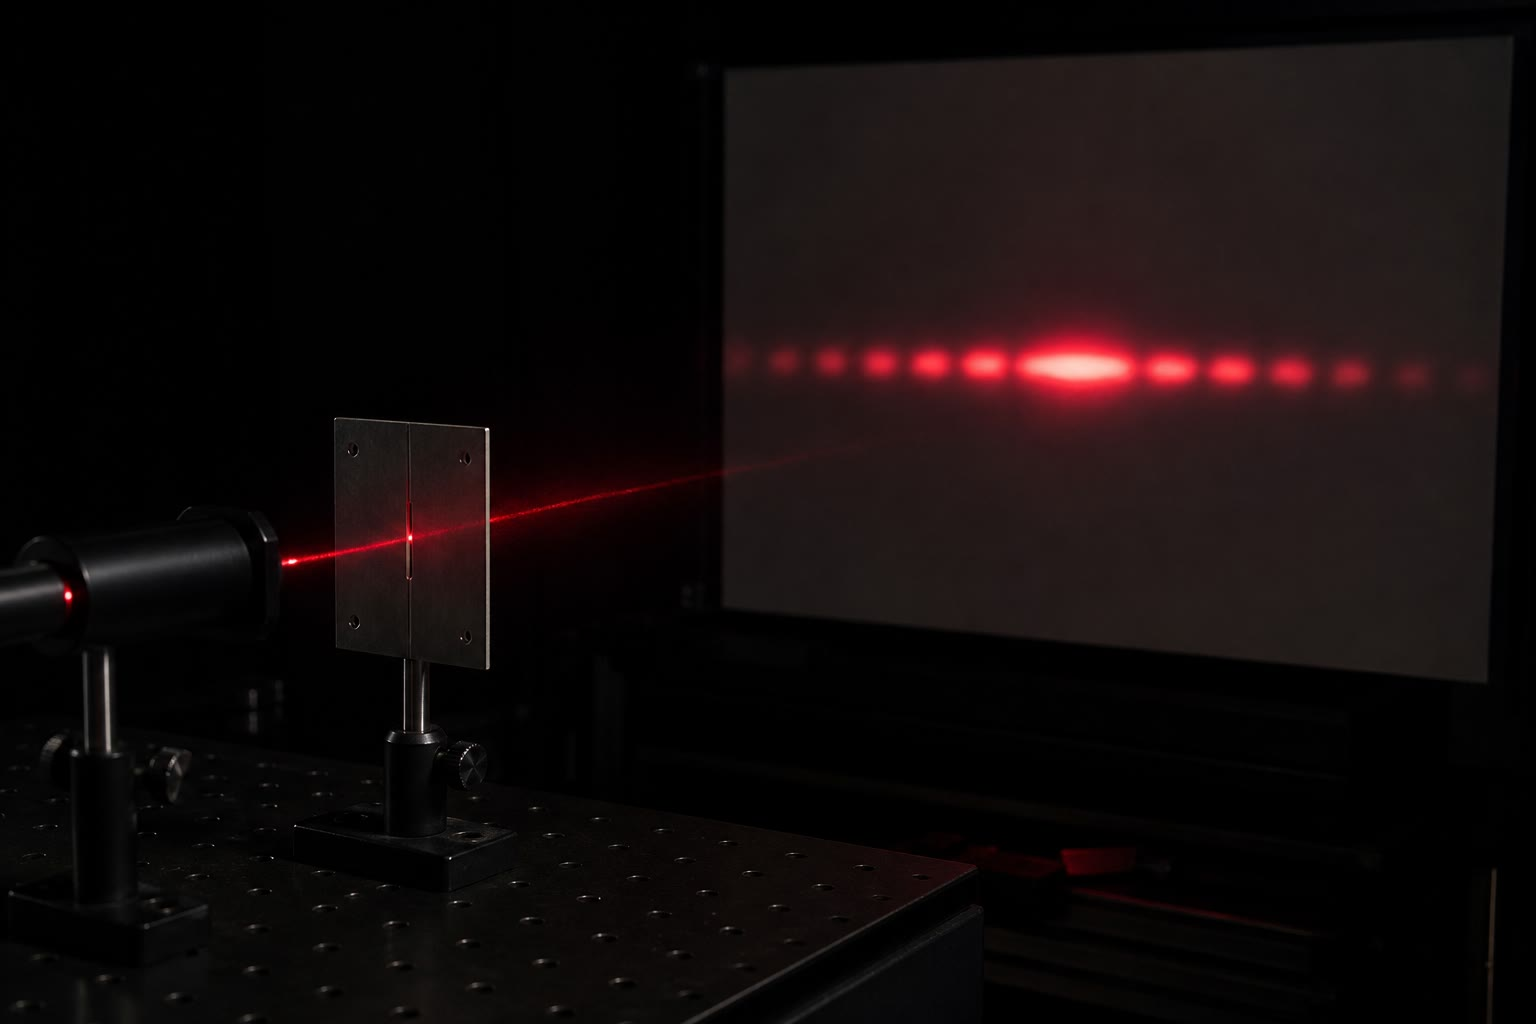
\includegraphics[width=0.58\linewidth]{images/book4/ai/b4-22-slit-diffraction-pattern.jpg}

{\small Un haz láser a través de una rendija estrecha: en la pantalla lejana, la ancha banda central brillante y los máximos laterales, más tenues y estrechos, del patrón de Fraunhofer.}
\end{omfigure}

\section{Problema: qué puede resolverse}

\begin{problem}[{Problema de fin de semana --- el límite de difracción a cuatro
escalas: el ojo, un telescopio, un microscopio y el haz láser que
hay que limpiar antes de usarlo}]
\label{pb:b2:diffraction:1}

\medskip
\noindent\textbf{Parte I --- El ojo.}
Pupila $D = \qty{3}{mm}$ de día y \qty{7}{mm} de noche; $\lambda = \qty{550}{nm}$; los
conos de la retina están separados \qty{2}{\micro m} en la fóvea, y la distancia focal
del ojo es de \qty{17}{mm}.
\begin{enumerate}
  \item Radio angular del \omterm{prop:b2:diffraction:airy}{disco de Airy} de día; su radio lineal en
        la retina; compárese con la separación de los conos --- ¿está la retina
        ajustada a la óptica?
  \item Menor separación de dos puntos resueltos a \qty{25}{cm}; y a
        \qty{10}{m}; ¿puede leerse un texto de \qty{1}{mm} con el brazo extendido?
  \item De noche la pupila se abre a \qty{7}{mm}: límite de \omterm{def:b2:diffraction:huygens}{difracción} entonces;
        ¿por qué empeora sin embargo la visión (aberraciones del
        cristalino a plena abertura, bastones más gruesos que los conos)?
  \item Dos faros de coche separados \qty{1.5}{m}: distancia a la que se funden
        en una sola luz.
  \item Un agujero de \qty{1}{mm} ante el ojo: ¿qué hace la \omterm{def:b2:diffraction:huygens}{difracción},
        y por qué ayuda sin embargo un agujerito a un ojo miope
        (profundidad de campo)?
\end{enumerate}

\medskip
\noindent\textbf{Parte II --- El telescopio.}
Un telescopio de \qty{1}{m}, $f = \qty{10}{m}$, con una cámara de píxeles de \qty{10}{\micro m};
$\lambda = \qty{550}{nm}$.
\begin{enumerate}[resume]
  \item Límite de \omterm{def:b2:diffraction:huygens}{difracción} en segundos de arco; radio de Airy en el
        detector; píxeles por \omterm{prop:b2:diffraction:airy}{disco de Airy}.
  \item La atmósfera difumina las imágenes hasta \qty{1}{''}: ¿cuánta
        resolución del telescopio se pierde? Diámetro de telescopio para el que
        el límite de \omterm{def:b2:diffraction:huygens}{difracción} iguala al seeing.
  \item La óptica adaptativa corrige la atmósfera a \qty{2.2}{\micro m}:
        límite de \omterm{def:b2:diffraction:huygens}{difracción} allí; ¿por qué es más fácil en el infrarrojo?
  \item Una estrella binaria con componentes separadas \qty{0.15}{''}: ¿se resuelve con
        óptica adaptativa a \qty{2.2}{\micro m}? ¿Y a \qty{550}{nm} desde el espacio?
  \item La Luna está a \qty{3.8e5}{km}: menor cráter que este telescopio
        podría resolver (solo por \omterm{def:b2:diffraction:huygens}{difracción}); ¿y la huella de un módulo
        lunar (\qty{4}{m})?
  \item Poder colector de luz del telescopio respecto del
        ojo nocturno (\qty{7}{mm}); ¿qué se gana con eso y qué no?
  \item La luz de una estrella a través de los cuatro brazos que sujetan el
        espejo secundario: descríbase la imagen.
\end{enumerate}

\medskip
\noindent\textbf{Parte III --- El microscopio.}
Objetivo de \omterm{prop:b2:guided-waves:fibre}{apertura numérica} $\mathrm{AN} = n\sin\alpha = 0.9$ (en seco) o $1.4$
(en aceite), $\lambda = \qty{550}{nm}$; la distancia resuelta vale $0.61\lambda/\mathrm{AN}$.
\begin{enumerate}[resume]
  \item Distancia resuelta con cada objetivo; número de pares de líneas
        por milímetro.
  \item Una bacteria de \qty{1}{\micro m} con estructura interna de
        \qty{0.2}{\micro m}: ¿qué se ve con cada uno? ¿Y un virus de \qty{0.1}{\micro m}?
  \item Abbe: una estructura periódica de periodo $d$ solo se imagina si sus
        primeros órdenes en $\sin\theta = \lambda/d$ entran en el objetivo: $d$ mínimo
        para $\mathrm{AN} = 1.4$; compárese con $0.61\lambda/\mathrm{AN}$.
  \item ¿Por qué mejora la resolución el aceite entre el portaobjetos y el objetivo?
  \item Ultravioleta a \qty{250}{nm} y un microscopio electrónico a \qty{4}{pm}:
        distancias resueltas con la misma fórmula (para los electrones la
        AN práctica es \qty{0.01}{}): compárense.
  \item Una célula es transparente: en campo claro su imagen está vacía.
        Explíquese en dos frases qué hace la lámina de contraste de fase en el
        \omterm{prop:b2:diffraction:fourier}{plano de Fourier} del objetivo.
\end{enumerate}

\medskip
\noindent\textbf{Parte IV --- El haz.}
Un láser de \qty{532}{nm}, con un haz de \qty{1.5}{mm} de diámetro, ha de expandirse a
\qty{30}{mm} y limpiarse.
\begin{enumerate}[resume]
  \item Semiángulo de \omterm{def:b2:diffraction:huygens}{difracción} del haz en bruto ($\sim1.22\lambda/D$); su
        diámetro tras \qty{100}{m} sin óptica alguna.
  \item Una lente de $f_1 = \qty{10}{mm}$ lo enfoca: diámetro de la mancha focal;
        diámetro de agujerito elegido ($1.5\times$ la mancha).
  \item Una segunda lente de $f_2$ recolima a \qty{30}{mm}: $f_2$; nuevo
        ángulo de \omterm{def:b2:diffraction:huygens}{difracción}; diámetro tras \qty{1}{km}.
  \item Un polvo de \qty{100}{\micro m} en la primera lente difracta ¿con qué ángulo?
        ¿Dónde cae esa luz en el plano del agujerito y qué
        le ocurre?
  \item El agujerito deja pasar el $99\%$ de un haz gaussiano: potencia perdida y
        a dónde va.
  \item ¿Por qué debe ser \emph{mayor} el haz expandido para seguir paralelo
        (relaciónese $\lambda/D$ con la distancia en la que el haz duplica su tamaño,
        $\sim D^2/\lambda$)?
  \item Resúmanse en una tabla los cuatro límites de este problema: abertura,
        longitud de onda, $\lambda/D$ y qué limita.
\end{enumerate}
\end{problem}
